\documentclass[conference]{IEEEtran}
\IEEEoverridecommandlockouts
% The preceding line is only needed to identify funding in the first footnote. If that is unneeded, please comment it out.
\usepackage[style=numeric]{biblatex}
\addbibresource{citations.bib}
\usepackage{amsmath,amssymb,amsfonts}
\usepackage{minted}
\usepackage{algorithmic}
\usepackage{graphicx}
\usepackage{listings}

\usepackage{textcomp}
\usepackage{xcolor}
\def\BibTeX{{\rm B\kern-.05em{\sc i\kern-.025em b}\kern-.08em
    T\kern-.1667em\lower.7ex\hbox{E}\kern-.125emX}}
\begin{document}

\title{Smart Parking Lot Assist System\\
{\footnotesize \textbf{
    Final Report \\
    Submitted in partial fullfilment of the requirements for senior design project\\
    Electrical and Computer Engineering Department \\
    Rutgers University, Piscataway, NJ 08854 \\
}
}
}

\author{
\textbf{Rajeev Atla, Parshva Mehta, Aman Patel, Abhiram Vemuri} \\
Advisor: Kristin Dana\\
Team Number: SP25-02 
}

\maketitle

\begin{abstract}
    As transport infrastructure grows increasingly complex, 
    large universities face increasing challenges in meeting the parking demands of students and faculty, 
    especially with continued reliance on personal vehicles. 
    Previous attempts to improve parking through automated valet systems have failed mainly due to high costs and logistical difficulties. 
    In campus environments, 
    shifting schedules and limited staff availability further complicate these solutions, 
    resulting in drivers often wasting time circling crowded lots, 
    causing congestion and increased emissions.
    This project introduces a scalable Smart Parking Assist System to address these issues that leverages computer vision and a web application to provide real-time parking detection and guidance. 
    The system comprises three core components: 
    the Machine Learning Model, 
    the Hardware Setup, 
    and the User Application.
    The machine learning component begins with dataset collection, 
    combining public datasets with images from the CoRE building. 
    These are preprocessed and then used to train a YOLO-based model capable of accurately classifying parking spaces. 
    The trained model weights are deployed to the hardware module.
    The hardware consists of a Raspberry Pi and a high-resolution camera capturing parking lot images and performing on-device inference. 
    Outputs are formatted as JSON and sent to the backend.
    The application includes both a frontend and a backend. 
    The backend converts JSON data to CSV, 
    updates a central database, 
    and connects to the frontend. 
    The frontend delivers real-time updates, 
    allowing users to locate available spaces efficiently.
    These components create a seamless, 
    scalable, 
    real-time parking solution suitable for university campuses and urban environments.    
\end{abstract}

\begin{IEEEkeywords}
    Computer Vision, Full-stack Development, Machine Learning, Data Pipelining/Manipulation
\end{IEEEkeywords}

\section{Introduction}
As transport infrastructure grows increasingly complex, 
large universities face mounting challenges in meeting the parking needs of students and faculty, 
especially with the continued reliance on individual car commuting. 
This project proposes an integrated solution using security camera imaging, 
computer vision, 
and a simple mobile application to ease the process of finding parking. 
The solution consists of two key components. 
First, 
a custom-configured security camera will be installed to overlook campus parking lots,
capturing high-resolution images. 
These images are processed through a computer vision model, 
pre-trained to detect open parking spaces with high accuracy. 
The output from this model is then converted into a dynamic dataset identifying available parking spots in real-time. 
Second, 
this dataset is seamlessly integrated into a user-friendly mobile application focused on clarity and ease of use. 
The app features an adaptive interface with real-time maps, 
filters, 
and notifications, 
enabling users to quickly locate free parking spaces near their destinations and make more informed parking decisions. 
Past attempts to improve parking with automated valet systems have failed, 
often because of high costs, 
complicated logistics, 
and issues with reliability. 
In a lively campus setting, 
these valet systems could be more feasible: 
changing class schedules, 
various modes of transportation, 
and limited staff availability make it hard to provide reliable valet services. 
As a result, 
drivers waste precious time driving in circles in busy lots, 
leading to congestion, 
frustration, 
and adverse environmental effects. 
By combining advanced imaging technology with intuitive design, 
this project aims to enhance the daily commuting experience for students and faculty. 
Moreover, 
integrating this information into an accessible platform contributes to the broader goal of fostering sustainable and efficient urban mobility patterns, 
paving the way for data-driven transportation solutions on and beyond university campuses.

\section{Approach Methods}

\subsection{Dataset Prep}

The foundation of this project lies in a diverse and robust dataset composed of parking lot images that represent a wide range of occupancy conditions. 
This dataset is publicly accessible through the GitHub repository maintained by Kimia-CVEngineer \cite{dataset_images}, \cite{images_original}, 
and it serves as a critical asset for the development and evaluation of our parking space detection system. 
The dataset is extensively annotated using structured metadata that clearly identifies each individual parking space within the images and labels them according to their occupancy status—either occupied or vacant. 
These labels are provided in a format compatible with common computer vision training pipelines, 
enabling seamless integration with object detection frameworks such as YOLO. 
The presence of accurate and consistent annotations eliminates the need for manual labeling and significantly accelerates the development process, 
while also ensuring that the data used for training reflects real-world parking behaviors and layouts. 
As such, 
this annotated dataset offers a reliable foundation for supervised learning and model benchmarking tasks.

The images included in the dataset are collected from various public sources, 
encompassing different parking lot configurations, 
environmental contexts, 
and camera viewpoints. 
This diversity is a key strength, 
as it helps the model learn to recognize parking spaces under numerous conditions, 
including varied lighting, 
differing camera angles, 
obstructions, 
and vehicle types. 
For example, 
some images are taken in outdoor lots during daylight hours,
while others may depict indoor structures with artificial lighting or nighttime scenes. 
Additionally, 
the dataset includes images from both compact and large-scale parking facilities, 
capturing parallel, 
perpendicular, 
and diagonal parking orientations. 
To complement this diversity and enhance the system’s applicability to our deployment environment, 
we also integrate proprietary images captured using our own custom-built camera system. 
These images are collected under controlled conditions that reflect the specific characteristics of the locations where the detection system is intended to operate, 
including unique layouts, signage, 
and vehicle patterns. 
By combining public and proprietary data, 
we create a hybrid dataset that is both comprehensive and contextually relevant, 
improving the model’s ability to generalize and adapt to real-world conditions.

To prepare the dataset for use in training and inference, 
we apply a series of preprocessing steps designed to standardize and enhance the input images. 
First, 
each image is resized to a fixed resolution compatible with the requirements of the neural network architecture. 
This ensures uniformity in input dimensions and reduces computational load during training. 
Next, 
pixel intensity normalization is performed to bring all image values into a common range, 
which helps stabilize gradient descent during backpropagation and leads to faster convergence. 
In addition to these standard steps, 
we employ a range of data augmentation techniques that artificially expand the size and diversity of the dataset.
These include horizontal and vertical flipping, 
brightness and contrast adjustments, 
random cropping, 
rotation, 
scaling, 
and the addition of noise or simulated occlusions. 
Such augmentations are essential for improving the model’s robustness to real-world variations such as changes in weather or time of day. 
Collectively, 
the preprocessing pipeline enhances both the quality and diversity of the data, 
ensuring that the model is trained on images that reflect the full range of conditions it may encounter during actual deployment.

\subsection{ML Model}

This project leverages the YOLOv11 
(You Only Look Once) 
object detection algorithm \cite{yolo11_ultralytics}
as the core of its parking space detection system. 
YOLOv11 represents a cutting-edge evolution of the YOLO architecture, 
offering a powerful balance between detection accuracy and computational efficiency. 
It is particularly well-suited for real-time applications such as intelligent transportation systems and smart parking solutions, 
where rapid inference and minimal latency are essential. 
YOLOv11 introduces enhancements over previous versions, 
including improved anchor-free object detection, 
better spatial understanding through transformer-based modules, 
and a more efficient feature pyramid network for multi-scale detection \cite{yolo11_overview}. 
These improvements make it capable of accurately identifying both small and large objects within cluttered scenes, 
which is crucial when detecting parked vehicles that may appear at different scales and levels of visibility within a single image.

To tailor YOLOv11 for the specific challenges of parking space detection, the model is extensively fine-tuned using the annotated dataset \cite{dataset_images}
described earlier. 
This fine-tuning process addresses key domain-specific issues such as variability in vehicle types, 
differing parking layouts, 
and complex visual obstructions. 
For instance, vehicles may partially extend outside parking boundaries, 
be parked at awkward angles, 
or be obscured by environmental factors such as shadows, 
rain, 
or nearby foliage. 
The training pipeline integrates advanced image processing techniques to maintain detection reliability across such diverse scenarios including,
contrast normalization, 
histogram equalization, 
and dynamic augmentation based on weather or lighting conditions. 
These steps enhance the model’s resilience in real-world settings.

\subsection{Hardware}

Selecting the Raspberry Pi 5 and a compatible camera module plays a key role in the success of this project. 
The Raspberry Pi 5 provides the necessary processing power and connectivity to support smooth, 
stable operation of the machine learning model without outages or connection issues. 
A secure mounting system ensures the camera remains in a fixed position, 
producing consistent image captures critical for accurate detection. 
The testing phase evaluates the system’s hardware stability, 
image quality, 
and model performance across various parking lot layouts. 
Extensive field testing helps fine-tune the integration and optimize the system for real-world deployment. 
In cases where the Raspberry Pi 5 cannot handle full model inference locally due to computational limits, 
the system is configured to offload processing to an external computer. 
In such setups, 
the Raspberry Pi 5 transmits images over Wi-Fi or Ethernet, 
maintaining its role as the edge capture and communication device.

\subsection{Software}

The software component of the system integrates advanced image processing, 
machine learning, 
and user-facing features to deliver a complete and user-friendly parking detection solution. 
When the camera system captures images, 
they first pass through a series of preprocessing steps designed to optimize visual quality. 
These steps include noise reduction to eliminate unwanted artifacts, 
color correction to maintain visual consistency across various lighting conditions, 
and general image enhancement to bring out features relevant to the model’s analysis. 
These refinements ensure that the inputs fed into the trained model are clean, 
well-structured, 
and highly representative of real-world scenes, 
thereby boosting detection reliability. 
Once the images have been preprocessed, 
they are passed through the inference pipeline, 
which utilizes the YOLOv11 model to detect and classify parking spaces in real time. 
The system is designed to deliver results with minimal delay, 
ensuring that parking availability data remains accurate and actionable. 
The system relies on robust data transmission protocols such as Wi-Fi or cellular networks, 
allowing it to connect with central servers or user devices without interruption. 
This seamless flow of information is essential for maintaining synchronization between edge devices and the broader application ecosystem.

The web application serves as the central user interface, 
providing a visually rich and interactive experience for users needing real-time parking availability updates. 
The application is designed to be functional and easy to navigate, 
with tools allowing users to view parking lots in map format, 
search for specific locations, 
and receive live notifications when spaces become available. 
Available parking spots are clearly marked and visually distinguished, 
helping users identify open spaces quickly and without confusion. 
This clear visual feedback reduces the time spent searching for parking and enhances overall user satisfaction. 
The system is built so that the outputs from the machine learning model are efficiently transmitted to the app’s backend, 
where they are interpreted and converted into meaningful updates. 
These updates are then displayed on the front-end interface in near real time, 
ensuring that users always have access to the most current parking status. 
The application strongly emphasizes user experience by incorporating a responsive design that functions smoothly across smartphones, 
tablets, 
and desktops. 
This ensures that users can access the system wherever they are, 
using the most convenient device, making the solution practical and accessible for daily use in a wide variety of scenarios.

\section{Challenges}

Throughout the development of our project, we encountered several significant challenges related to regulation and the supply chain, which ultimately limited the performance, timeline, and scope of our system. From the outset, our team had a clear and ambitious vision for how the system would function, with specific technical goals and hardware placements in mind. One of the key foundational elements of our original design was the use of an aerial camera perspective. This choice was heavily informed by the dataset images we trained on (see Figure 4), which provided a high-angle view that clearly delineated parking lines and allowed bounding boxes to be easily drawn around each space. These images offered the ideal conditions for our machine learning model to perform effectively, as the clear view from above minimized visual obstructions and provided a consistent and comprehensive layout of the parking area.

However, despite the clarity of our technical vision, we were soon faced with unforeseen regulatory constraints imposed by Rutgers University and the State of New Jersey. These regulations prohibited the installation of cameras on elevated platforms or the use of drones, which had been central to our original plan. The restrictions were rooted in concerns related to safety, privacy, and compliance with institutional and state policies, all of which were beyond our control. As a result, our team was forced to reevaluate and revise our approach in order to comply with these constraints. Ultimately, we decided to place a stationary camera on the 5th floor of the CoRE building, which provided a fixed perspective of the parking lot. While this solution allowed us to move forward with implementation, it introduced a new set of challenges. Unlike the clean, overhead view provided by aerial imagery, the 5th-floor angle from the CoRE building resulted in partial obstructions, as many parking spots were blocked by larger vehicles parked in front of them. This significantly reduced the visibility and clarity of the images captured, which in turn affected the reliability of the inputs fed into our machine learning model.

Compounding these challenges were supply chain issues that further disrupted our timeline. Several essential hardware components, specifically the camera’s power supply and SD card, arrived later than expected, near the end of the semester, despite having been ordered well in advance. These delays significantly hindered our ability to set up the system in the intended on-site environment. Without these components, we were unable to fully configure and test the camera on location, meaning we had limited access to real-world data from our designated parking lot. The inability to collect this crucial data during key stages of development had a direct impact on the training and performance of our machine learning model. The model's accuracy and effectiveness depend heavily on being trained and tested with consistent, high-quality inputs from the actual deployment environment, and unfortunately, this was not possible within our original timeframe.

The late arrival of these components had a cascading effect on the rest of the project. Our goal had been to build a fully integrated system where the camera would capture continuous video, the YOLOv11 model would be deployed on a Raspberry Pi for local inference, images with bounding boxes would be stored and analyzed, and relevant data would be pushed to a database. This database would then be used to update a user-facing website, providing real-time insights into parking availability. However, due to the absence of the camera’s power supply and SD card for a substantial portion of the semester, our ability to test and refine this pipeline in a real-world setting was severely limited.

On the software side of the project, the absence of working hardware meant we had to implement a temporary workaround in order to continue development. To simulate the camera input, we resorted to using our mobile phones to capture footage of the parking lot. While this allowed us to collect some data and test portions of the pipeline, it came with significant drawbacks. The mobile phone footage lacked the consistency and quality of a dedicated surveillance camera. Differences in resolution, unstable frame rates, and varying lighting conditions made it difficult for the machine learning algorithm to perform as effectively as it could under ideal conditions. This inconsistency resulted in lower confidence detections, and occasionally, the algorithm would miss or mislabel parking spaces as occupied or vacant. These inaccuracies, in turn, led to flawed outputs in the resulting CSV file, which was then used to update the database. As a consequence, some false positives and incorrect entries were introduced, affecting the overall reliability of the system.

In addition to data quality issues, another complication we encountered involved optimizing how frequently the database should be updated. Initially, our system was configured to update the database every 5 to 10 seconds based on new outputs from the CSV file. While this approach aimed to provide near real-time data, it soon became apparent that such a high refresh rate introduced several unintended consequences. The backend system began to experience database locking issues and writing conflicts. Occasionally, the server would even crash when attempting to process simultaneous requests from the frontend. These performance bottlenecks were disruptive and made it difficult to maintain a stable and functional platform for users. To address this, we adjusted the refresh interval to 30 seconds, which significantly improved system stability. With more time between updates, the backend had the breathing room it needed to process images more thoroughly, reduce conflicts with frontend requests, and generate more accurate outputs. While this slightly reduced the immediacy of updates, it offered a more sustainable and reliable approach to system performance, balancing the need for timely information with technical feasibility.

In summary, while the project faced several unforeseen setbacks, including regulatory restrictions and delays in hardware delivery, we adapted our approach and found creative workarounds to continue progress. These experiences taught us valuable lessons in project management, systems integration, and real-world deployment challenges. Although the final implementation did not fully match our original plan, the modified system still demonstrated a functional and practical solution for detecting and reporting parking availability, an accomplishment made more meaningful by the hurdles we overcame along the way.


\section{Results}

During the model training phase, 
a fine-tuning strategy was adopted to navigate the uncertainty surrounding the optimal number of training epochs. 
Without explicit prior knowledge about when the model would converge to its best performance, 
we implemented a staged training process designed to refine the model's performance iteratively. 
Initially, 
the model was trained for a predetermined number of epochs to generate a foundational set of weights. 
These weights were then preserved and used to reinitialize the model for additional training cycles. 
By doing so, 
we allowed the model to build upon previously learned features and patterns, 
gradually improving its detection capability with each iteration. 
This stepwise refinement enabled us to more effectively balance the trade-off between underfitting, 
where the model fails to capture the complexity of the data, 
and overfitting, 
where the model becomes overly tailored to the training set and loses generalization ability.

Throughout this multi-stage training process, 
close attention was paid to key performance indicators, 
particularly the training and validation loss values. 
After each training cycle, 
the loss curves were carefully analyzed to assess the model's learning dynamics and convergence behavior. 
These plots serve as critical diagnostic tools, 
offering valuable insight into whether the model is continuing to improve, 
plateauing, 
or beginning to overfit. 
A steady decline in training and validation loss typically suggests that the model is learning effectively, 
whereas divergence between the two can indicate overfitting or poor generalization. 
By evaluating these trends at every stage, 
we were could make informed decisions about whether to continue training, 
adjust hyperparameters, 
or modify the dataset through augmentation or filtering.

This analytical approach provided a strong empirical foundation for guiding the model’s development, 
allowing for incremental yet meaningful improvements in performance. 
It also ensured that the final model was accurate in terms of detection metrics and stable and reliable across various testing scenarios. 
The insights gained from loss curve evaluations were instrumental in achieving a well-balanced model capable of generalizing to new, 
unseen parking lot images, 
further validating the effectiveness of the training methodology.


\subsection{Training Loss}

Figure \ref{fig:fig1} illustrates the progression of the training loss throughout the training process, offering a visual representation of how the model’s performance evolved over time. During the initial training epochs, the training loss displays noticeable fluctuations as the optimizer begins interacting with the data and adapting to the model’s initial parameter values. These fluctuations are a normal part of the learning process and reflect the model's early attempts to make sense of complex patterns in the training dataset. As the optimizer updates the weights based on feedback from the loss function, the model begins to adjust its internal representations and gradually learns to minimize the loss. This early instability signals the beginning of meaningful learning, during which the model makes rapid strides in performance.

The larger fluctuations observed during the early stages of training suggest that the model was learning quickly, likely due to a relatively high learning rate at the outset. These steep declines in the loss value indicate that the model effectively captured general trends in the data and made substantial progress toward better accuracy. A noticeable shift occurs: the loss curve stabilizes and follows a smoother downward trend. Around epochs 750 to 800, the curve enters a plateau phase, where the loss levels off and remains relatively constant at approximately 0.6. This leveling out suggests that the model is approaching convergence. At this stage, it becomes increasingly difficult for the optimizer to make large improvements, as the model’s parameters have settled into configurations that yield consistent performance on the training data.

The slight oscillations that appear during this plateau phase, often visualized as small “spikes” in the loss curve, correspond to moments of fine-tuning. These subtle fluctuations indicate ongoing adjustments by the optimizer to refine the model’s internal weights without causing significant disruptions to previously learned representations. These fine-tuning periods key to the training strategy, allowing the model to make small, targeted improvements. Rather than undergoing large-scale changes, the model adjusts incrementally, sharpening its understanding of nuanced patterns in the data. These spikes are expected and indicate that the training process is still active, albeit in a more refined and controlled phase.

The consistent rise and fall of the loss during each fine-tuning cycle highlights the adaptive and iterative nature of the training process. Importantly, each successive cycle results in a slightly lower final loss, demonstrating that these adjustments are successfully enhance the model’s accuracy. This pattern shows that the training strategy is effective in preventing overfitting and actively guiding the model toward better performance. Overall, the steady downward trend and eventual stabilization of the training loss reinforce the conclusion that the model is capable of learning efficiently and converging toward an optimal set of parameters suitable for parking space detection.


\begin{figure}[h]
    \centering
    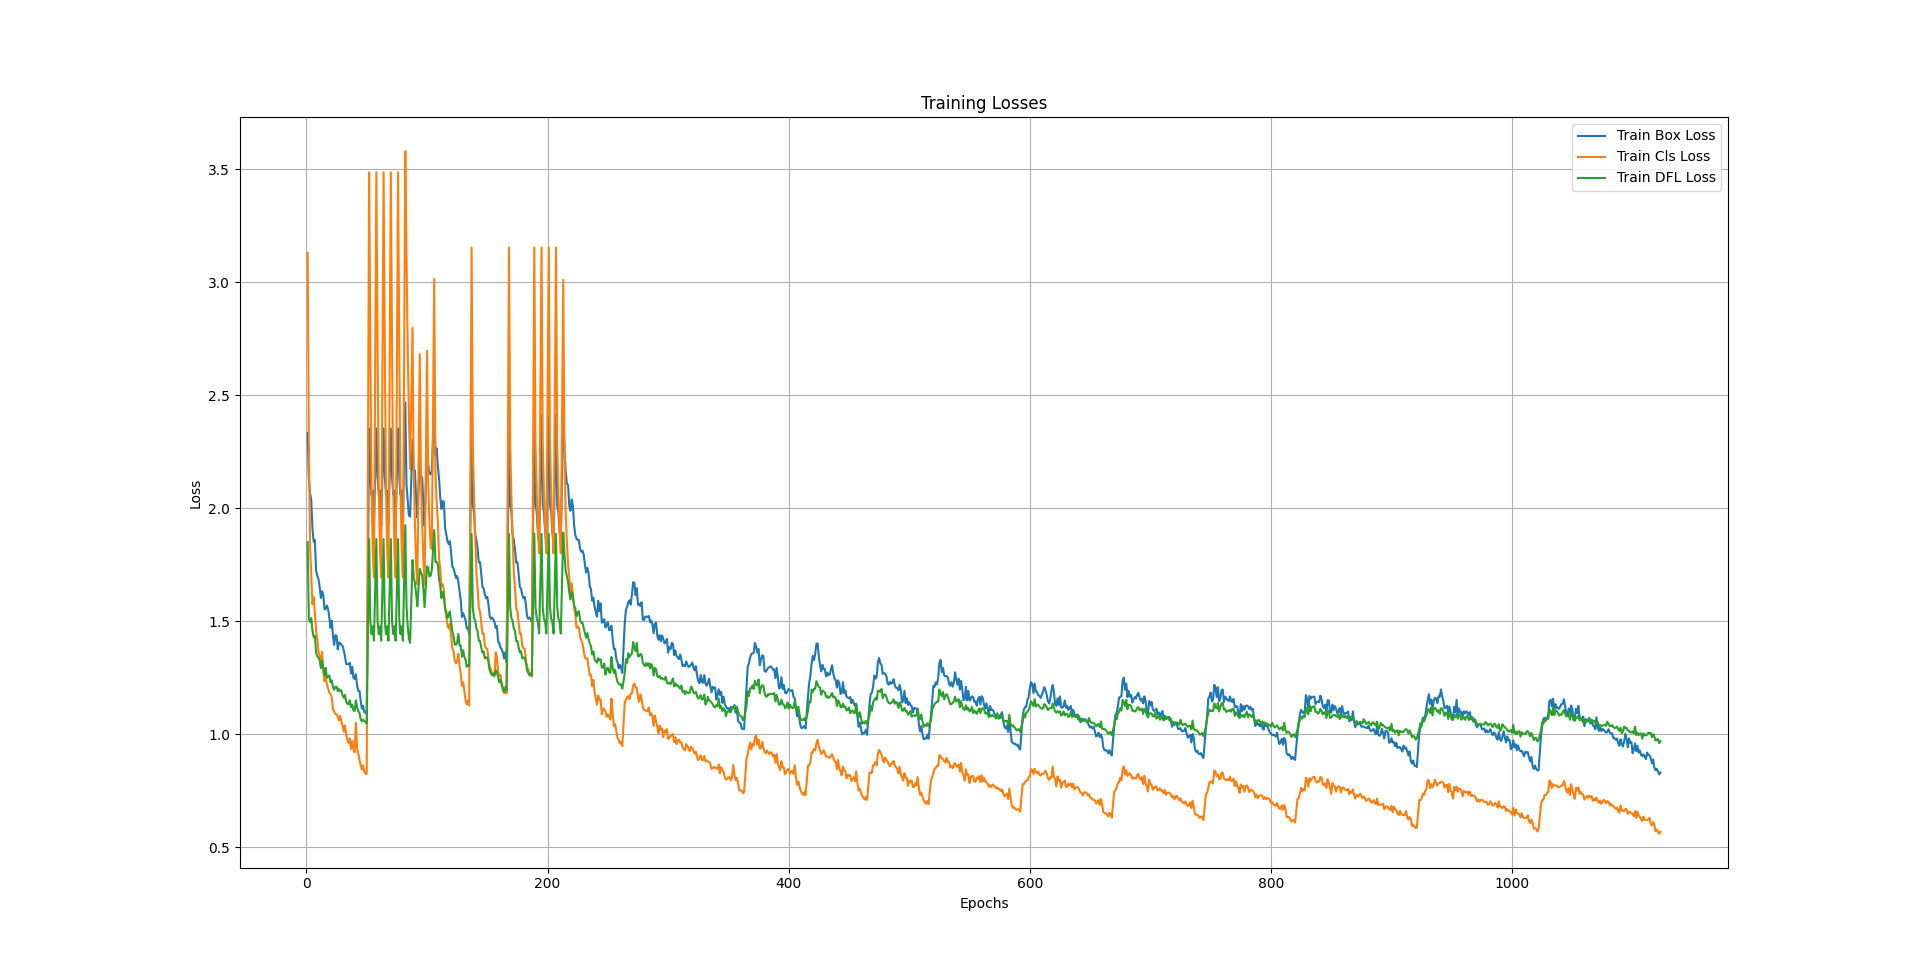
\includegraphics[scale=0.2]{Figure_1.png}
    \caption{
        Notice how the training loss generally decreases throughout the training and plateaus after 750-800 epochs at a value of 0.6. 
        The ''spikes'' in the beginning and throughout the plot represent fine-tuning.
    }
    \label{fig:fig1}
\end{figure}

\subsection{Validation Loss}

Figure \ref{fig:fig2} illustrates the progression of the validation loss throughout the training process, providing insight into how well the model performs on unseen data over time. In the initial stages of training, the validation loss decreases at a steady and consistent rate, closely mirroring the behavior observed in the training loss curve. This early improvement suggests that the model is not only fitting the training data but is also successfully capturing generalizable patterns that apply beyond the specific examples it has seen. As training progresses, however, the rate of improvement gradually slows. Around epochs 750 to 800, the validation loss begins to level off, forming a plateau that signals the model is reaching a point of diminishing returns. This flattening of the curve suggests that further training would result in only marginal gains and that the model’s performance has largely stabilized regarding its generalization ability.

Similar to the training loss, the validation loss curve also features small spikes and fluctuations, which are particularly noticeable during the plateau phase. These momentary increases in loss correspond to intervals of fine-tuning, where the optimizer continues to make subtle adjustments to the model's parameters in pursuit of better generalization. Although these fluctuations may appear as temporary setbacks, they are part of a normal and beneficial process that helps the model refine its internal representations. These slight variations reflect the dynamic nature of learning, where the optimizer carefully balances stability with the need to explore the parameter space for further improvements. Notably, the overall trajectory of the validation loss remains downward or stable, indicating that the model is not overreacting to individual data points and is maintaining its focus on broader generalization.

The clear plateau in validation loss observed after approximately 750 to 800 epochs marks an important transition in the training process. The model has reached a stable state where continued training could potentially lead to overfitting, as additional adjustments may begin to tailor the model too closely to the training data at the expense of performance on unseen inputs. Recognizing this, the decision was made to halt training at this point in order to preserve the model’s generalization capability. The behavior shown in the validation loss curve confirms the success of this approach, as it demonstrates that the model was able to reach optimal performance without excessive training. Overall, the validation loss trend supports the conclusion that the training process was well-controlled and effective in producing a robust and generalizable model.


\begin{figure}[h]
    \centering
    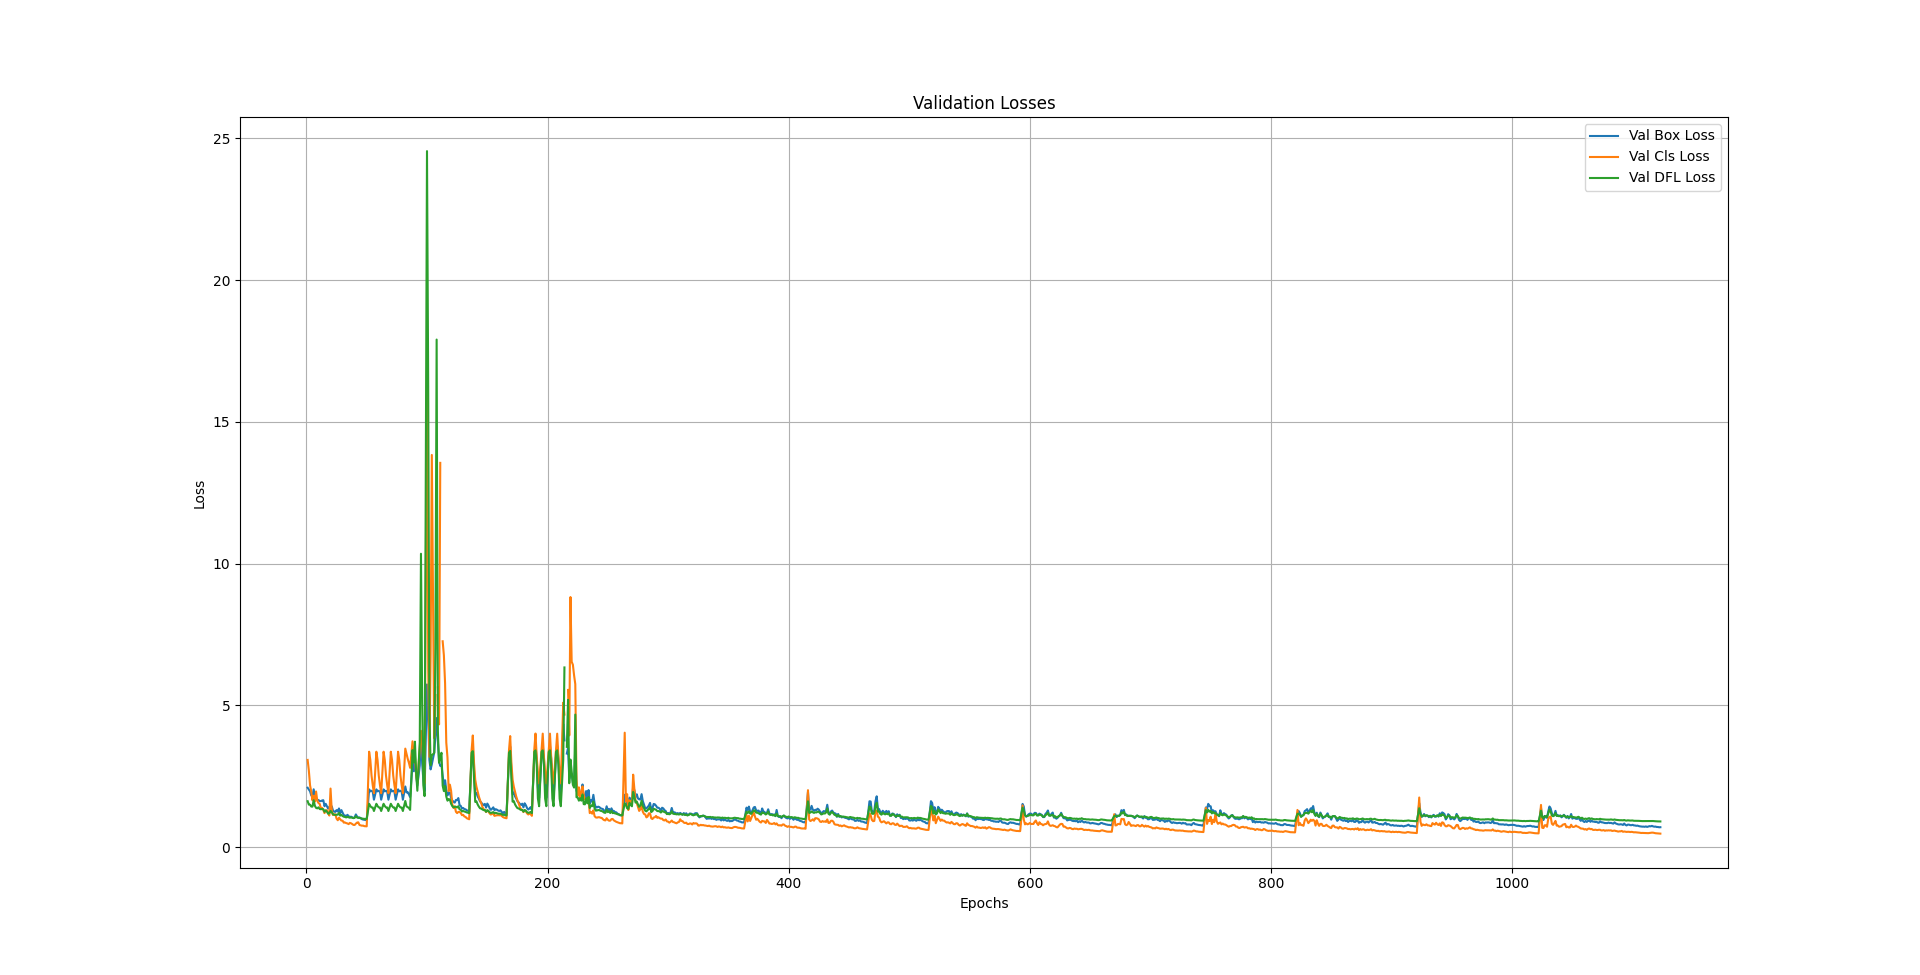
\includegraphics[scale=0.2]{Figure_2.png}
    \caption{
        Notice how the validation loss generally decreases and plateaus after 750-800 epochs. 
        When training the model, 
        the stopping point was when the validation loss plateaus. 
        The spikes are present in this plot as well.    
    }
    \label{fig:fig2}
\end{figure}

\subsection{Evaluation}

Figure \ref{fig:fig3} presents a comprehensive view of the evolution of the four key evaluation metrics used to assess the performance of our object detection model throughout the training process: Precision (P), Recall (R), mAP50 (Mean Average Precision at 50\% IoU threshold), and mAP50-95 (Mean Average Precision averaged across multiple IoU thresholds). As illustrated in the figure, the values of all four metrics show a consistent upward trajectory over time, indicating that the model is learning effectively from the training data and gradually improving its ability to detect objects accurately.

Precision, which measures the accuracy of the model’s positive predictions, exhibits a steady and promising increase throughout training. By the end of the process, it reaches a final value of approximately 0.87. This strong result reflects the model's growing capability to identify true positive detections while minimizing false positives correctly. In other words, when the model predicts that an object is present in a given location, it is increasingly likely to be correct. This is an essential quality in any object detection system, particularly one deployed in real-world environments where high accuracy is critical.

Recall, another vital metric, measures the proportion of actual positive cases the model successfully identifies. This metric also shows a consistent upward trend, ultimately reaching around 0.80. This increase demonstrates the model’s growing ability to identify a larger share of objects in the images. Practically, this means fewer objects are being missed as training progresses. Together, the increases in both precision and recall highlight the model’s balanced improvement in detecting objects accurately and comprehensively.

The two mAP metrics, mAP50 and mAP50-95, further reinforce the overall progress the model is making. These metrics are widely recognized as robust indicators of object detection performance, accounting for precision and recall across various detection thresholds. The mAP50 metric, which is generally considered the baseline for object detection accuracy, climbs steadily to finish at approximately 0.90. This high score reflects the model’s strong performance in detecting objects with reasonable spatial accuracy. Meanwhile, the mAP50-95 metric, which is more stringent due to its requirement for accuracy across a range of Intersection over Union (IoU) thresholds, concludes at a solid 0.72. This result indicates that the model is effective in general and increasingly capable of handling more challenging detection scenarios that demand greater precision in localization.



\begin{figure}[h]
    \centering
    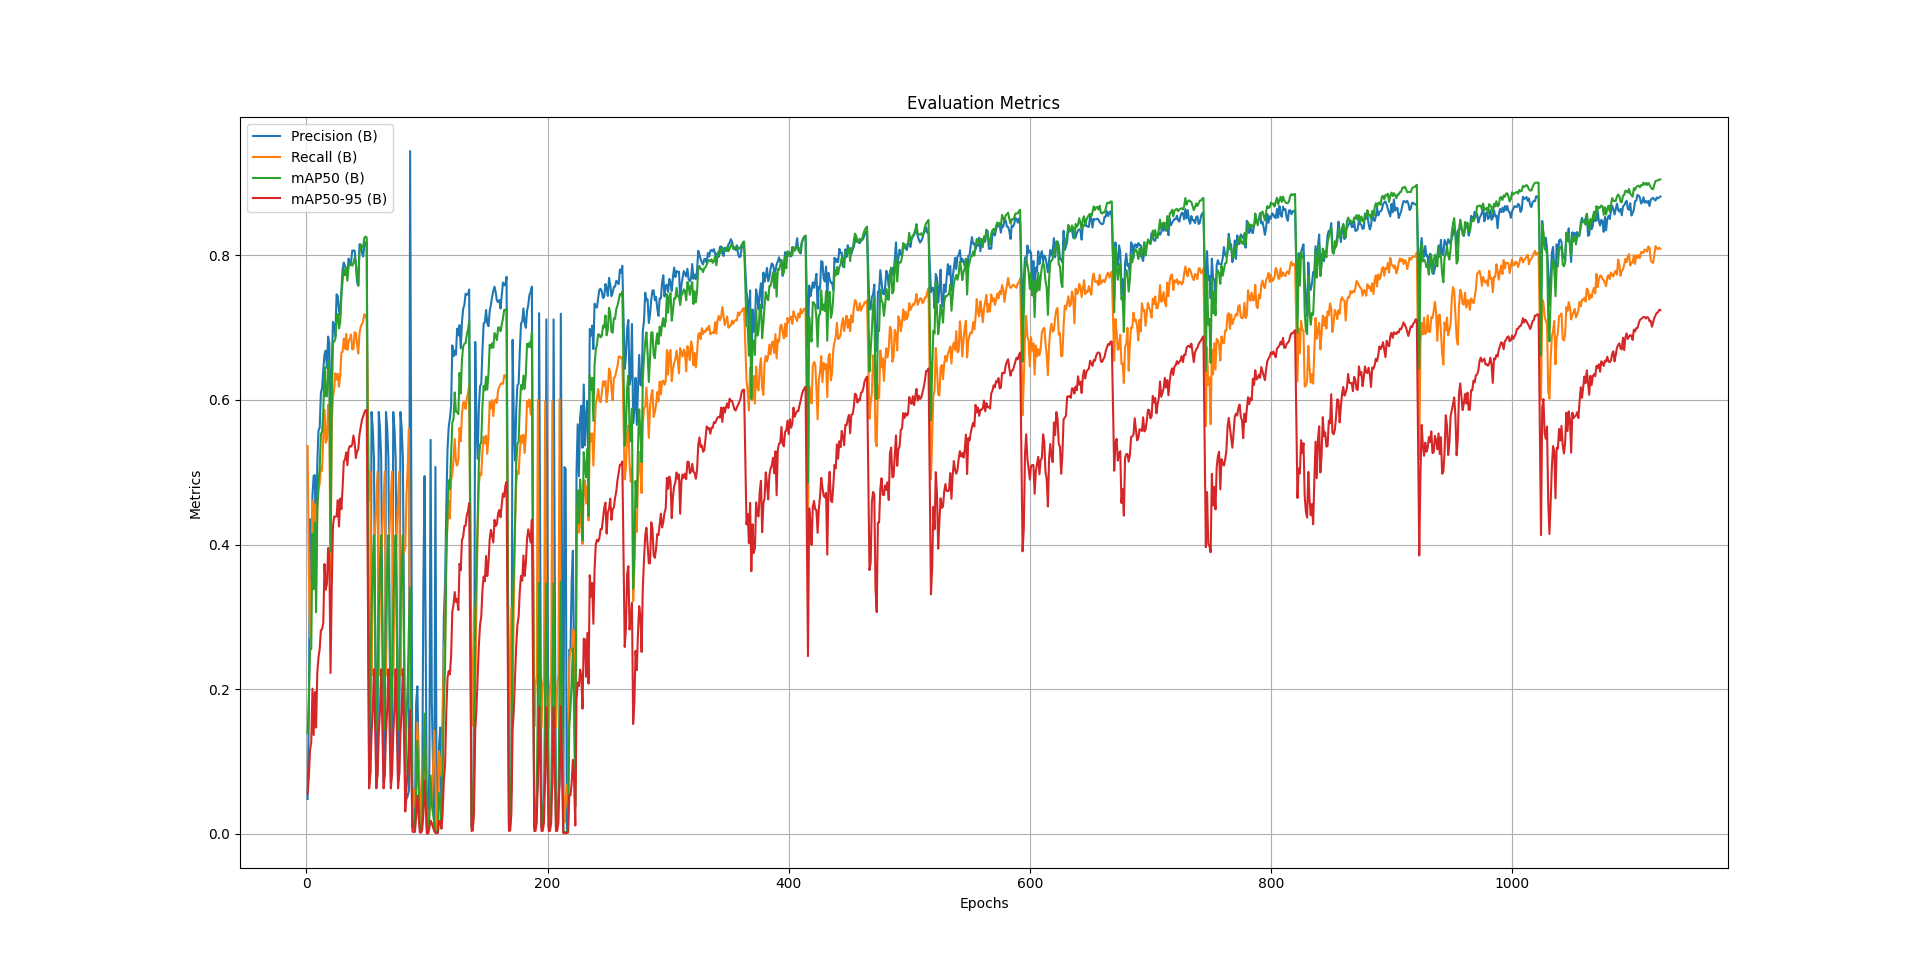
\includegraphics[scale=0.2]{Figure_3.png}
    \caption{
        The values of the four evaluation metrics 
        (Precision, Recall, mAP50, and mAP50-95) 
        improve steadily throughout the training process, 
        indicating that the model's performance enhances as training progresses. 
        The spikes in the plot reflect periods of fine-tuning and adjustments to the model’s weights.   
    }
    \label{fig:fig3}
\end{figure}

Figures 1, 
2, 
and 3 showcase the quantitative performance data of the machine learning model and provide valuable insights into its effectiveness and efficiency. 
By examining these plots, 
we can assess how the model's performance evolves over time, 
identify potential weaknesses or areas for improvement, 
and determine its ability to unseen data. 
Additionally, 
the plots reveal trends in the model's learning process, 
such as whether it is overfitting or underfitting. 
These quantitative metrics are essential for validating the model’s utility in real-world applications and guiding further refinement, 
ensuring that the model meets the desired standards for accuracy and reliability in tasks like parking space detection or any other specific objectives.


\subsection{Test Examples}

In Figure \ref{fig:fig4}, we present a test image from the dataset with bounding boxes overlaid to illustrate the model’s detection results. In this visual example, empty parking spaces are highlighted with green bounding boxes, signaling areas available for parking. In contrast, occupied spaces are marked in red to indicate that they are currently taken. The image clearly represents the YOLOv11 model’s ability to effectively distinguish between different types of parking space occupancy based on visual cues from the input data. The bounding boxes are cleanly aligned with the spaces in view, demonstrating the model’s detection accuracy and its consistency in classifying multiple parking spaces that are relatively close to the camera's position. This example captures one of the strengths of our system, its ability to provide quick and reliable visual outputs when the camera angle, resolution, and visibility conditions are favorable.

However, a contrasting scenario is presented in Figure \ref{fig:fig5}, where the model's limitations become more apparent. In this frame, which is taken from a test video rather than a static image, the camera captures a much wider field of view, including objects and parking spaces significantly farther from its position. In this case, the model encounters noticeable challenges in identifying and accurately classifying objects at greater distances. Vehicles and parking spaces that are further away appear smaller and less distinct, making it harder for the model to process them with the same level of accuracy as those closer to the camera. If present at all, the bounding boxes in this image are either misaligned or missing, indicating a drop in detection performance when resolution and visibility are compromised by distance.

This issue is common in real-world object detection systems, especially when working with large outdoor environments like parking lots, where the spacing between objects can vary greatly. As objects become more distant, they lose visual clarity, which reduces the amount of information available for the model to analyze. This diminished detail makes it difficult for the model to detect fine features, such as the outlines of a parking space or the shape of a vehicle, which are crucial for accurate classification. The test video frame in Figure 5 is a compelling example of this challenge and highlights the importance of strategic design considerations in system deployment.

Given this limitation, it becomes evident that relying on a single fixed camera, especially one positioned at a distance or high elevation, may not be sufficient to ensure complete and reliable coverage of an entire parking lot. This is especially true in lots with expansive layouts, multiple sections, or irregular configurations that introduce blind spots or areas of low visibility. To address this, one of the most practical solutions is to deploy multiple cameras at strategic points throughout the lot. By doing so, each section of the parking area can be monitored more closely and with greater resolution, helping to overcome the issues introduced by distance. With overlapping fields of view, these cameras can collectively provide comprehensive coverage and reduce the chances of missed or misclassified spaces.

Implementing a multi-camera approach improves the system’s spatial reach and enhances its reliability in varying lighting and environmental conditions. It allows the model to operate with clearer, more focused input images and helps ensure that detections remain consistent across the entire monitored area. In the context of our project, adopting such a configuration would be a meaningful step toward increasing the robustness and accuracy of the system, particularly in real-world applications where full situational awareness is essential.


\begin{figure}[h]
    \centering
    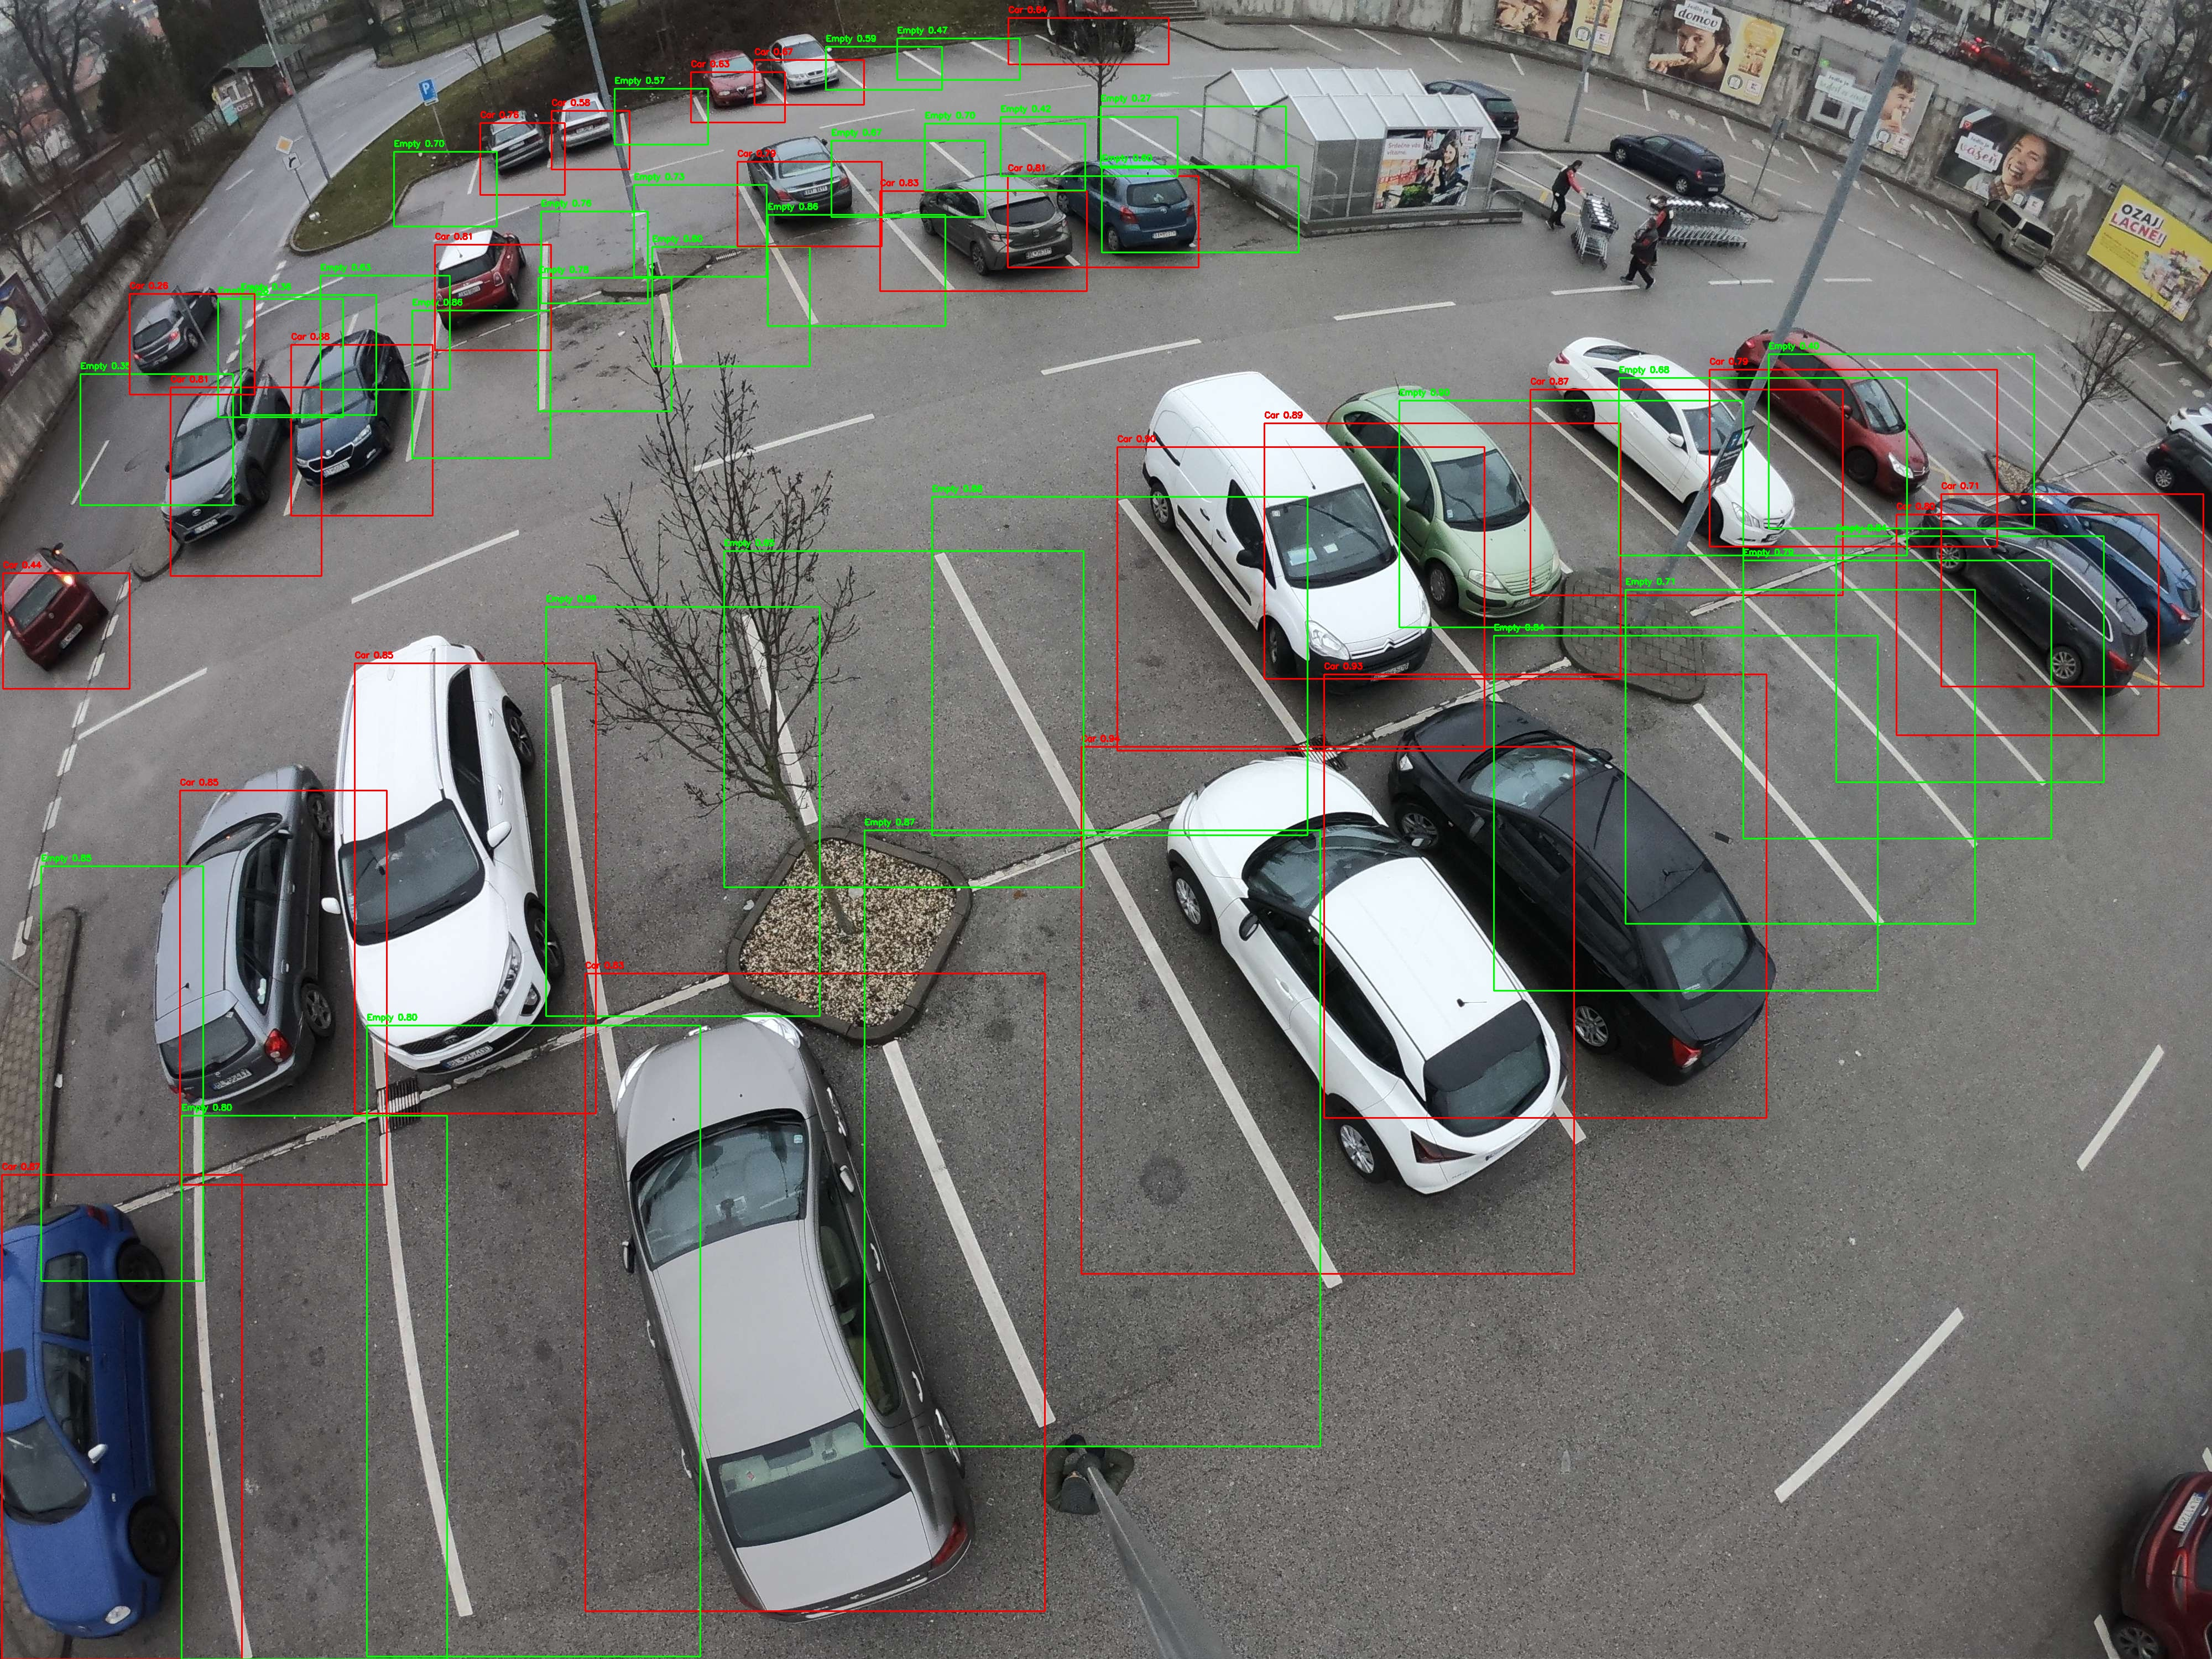
\includegraphics[scale=0.065]{Figure_4.JPG}
    \caption{
        Observe that the empty parking spaces are marked with green bounding boxes while occupied spaces are marked with red bounding boxes. 
        The YOLOv11 model correctly identifies and classifies spaces in the test data.
    }
    \label{fig:fig4}
\end{figure}

\begin{figure}[h]
    \centering
    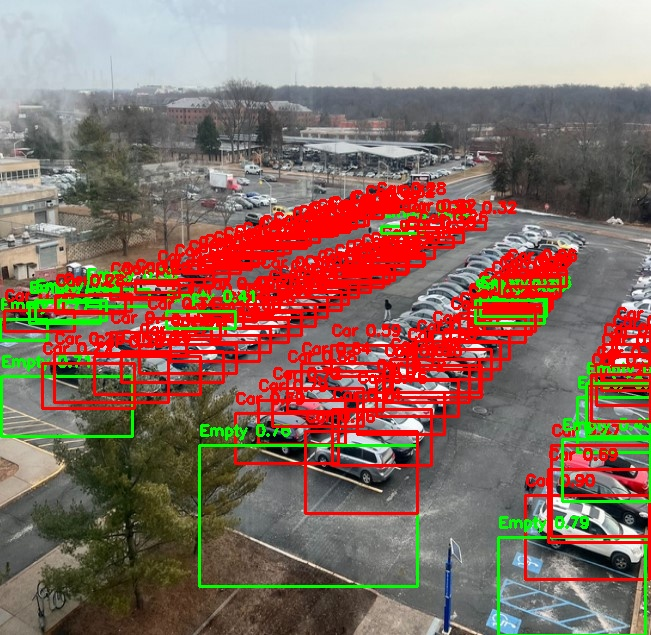
\includegraphics[scale=0.4]{Figure_5.JPG}
    \caption{
        Observe that the model struggles to identify vehicles and spaces at a distance. 
        Most lots will need more than one camera in order to cover every space. 
        This is a frame taken from a test video.   
    }
    \label{fig:fig5}
\end{figure}

Figures 4 and 5 are examples of qualitative data, 
which refers to non-numeric information that describes the characteristics or qualities of an object, 
phenomenon, 
or system. 
It can encompass user experiences or feedback regarding the ease of navigation within the parking lot, 
the availability of parking spaces during peak hours, 
or the overall safety and accessibility of the facility. 
Qualitative data is often subjective and focuses on the attributes or features that cannot be easily quantified but provide essential insights for improving the user experience, 
operational efficiency, 
and service quality. 
Figure 5 provides a visual example of the model working and finding open and closed parking spaces.

\section{Cost/Sustainability analysis}

This project involves developing an intelligent parking space detection system using a Raspberry Pi 5 (8GB) and a tilt-enabled camera setup. The system identifies empty and occupied parking spots to optimize parking efficiency and reduce time spent by drivers searching for available spaces. The prototype cost is approximately \$196.66, which includes the Raspberry Pi (\$80), tilt camera module (\$86.71), power supply (\$12), bumper (\$3), and a 64GB SD card (\$14.95). The estimated cost for mass production is approximately \$200 per unit, reflecting a cost-effective solution even at scale, especially considering its components' modularity and wide availability.

Economically, the project is designed with affordability and scalability in mind, making it a practical option for cities, private parking operators, and businesses seeking to modernize their infrastructure without incurring excessive expenses. The modest per-unit cost makes this system attractive, particularly when considering its long-term value. As demand increases, economies of scale could bring the production price down further, primarily through bulk purchasing agreements or partnerships with hardware vendors. Additionally, centralized data processing or cloud-based platforms could reduce the need for each camera to have its dedicated Raspberry Pi, further cutting down hardware and maintenance expenses. The overall system is structured to offer excellent value, with a low initial investment and reduced long-term costs thanks to its energy-efficient operation and minimal upkeep requirements.

Moreover, municipalities or organizations adopting this system may be eligible for government incentives to promote smart infrastructure and sustainable city initiatives. These may include grants, rebates, or tax breaks, especially in areas focused on lowering carbon emissions or deploying energy-efficient technologies. These financial advantages can make a significant difference in large-scale implementations, where tight budgets and return on investment are closely scrutinized. Beyond direct savings, the project also introduces indirect economic benefits. Minimizing the time drivers spend idling or circling in search of parking helps reduce fuel consumption and vehicle wear and tear, which translates into savings for individual drivers and reduced strain on urban roadways. Businesses in high-traffic areas may also benefit, as improved parking availability can increase foot traffic and customer satisfaction.

From an environmental standpoint, the system has the potential to generate a meaningful positive impact. One of the most pressing urban challenges is unnecessary vehicle emissions from prolonged searches for parking, which not only waste fuel but also contribute to air pollution and greenhouse gas buildup. The system actively reduces these emissions by streamlining the process and helping drivers find parking more efficiently. Its low-energy hardware and efficient power usage mean it operates sustainably and minimally impacts the environment. In future iterations, further green considerations such as solar-powered modules or eco-friendly enclosures could enhance the project's sustainability profile even more.

Socially, the system contributes to smarter and more livable cities by making a frustrating everyday task, finding a parking spot, more straightforward and predictable. This improvement in urban mobility reduces driver stress, increases satisfaction, and supports more harmonious traffic flow, particularly in densely populated or high-demand areas. Importantly, the system enhances accessibility by helping those with mobility challenges or disabilities find appropriate parking more easily, contributing to a more inclusive urban experience. While automation might reduce some roles traditionally filled by parking attendants, it also creates new opportunities in areas such as technology deployment, maintenance, and data management. These emerging roles align well with the growing demand for digital and infrastructure-focused careers and can contribute to local job creation.

The system may also support public safety initiatives. Reducing chaotic or illegal parking practices and improving overall organization can help prevent accidents and make parking areas safer for both drivers and pedestrians. Additionally, it aligns with the broader movement toward smart infrastructure that supports real-time responsiveness, data-driven planning, and environmental responsibility. As cities evolve, systems like this serve as building blocks for more connected, efficient, and sustainable urban environments.


\section{Computer Vision/Society}

The widespread adoption of machine vision technologies has transformed the landscape of urban infrastructure, placing robotics at the heart of contemporary societal innovation. 
These vision-based systems are foundational to the development of smart cities, 
enabling a range of applications from traffic management and surveillance to public service automation. 
By offering real-time visual interpretation, 
machine vision equips autonomous systems with the capability to interact meaningfully with dynamic environments. 
This capability enhances urban operations' efficiency, 
sustainability, 
and safety, 
creating more responsive and adaptive cities. 
Integrating these systems into daily infrastructure allows for continuous monitoring and intelligent decision-making, 
ultimately improving the quality of urban life.

Recent technological advances have made it possible to implement vision-based object detection and tracking using efficient and lightweight methods. 
For instance, 
techniques that utilize frame differencing, 
adaptive thresholding, 
and computationally simple tracking algorithms have been shown to detect moving objects in real time with minimal resource requirements, 
as discussed in \cite{wang_and_zhang}. 
These approaches are particularly valuable in settings when hardware limitations or cost constraints are a concern, 
offering affordable yet effective alternatives to more complex and hardware-intensive systems. 
In parallel, 
deep learning methods, 
particularly those based on convolutional neural networks, 
have greatly improved the accuracy and responsiveness of object detection systems. 
Models like YOLO exemplify this progress by achieving a balance between inference speed and detection accuracy, allowing real-time application in a range of real-world scenarios.

One domain where these technologies have had a pronounced impact is in urban mobility, 
primarily by deploying smart parking systems. 
The study presented in \cite{smart_parking} 
illustrates how machine vision can be employed to identify and classify parking spaces, 
thereby reducing traffic congestion, 
lowering emissions from idling vehicles, 
and improving the overall efficiency of urban space utilization. 
By continuously monitoring parking availability and conveying that information to users, 
such systems streamline parking behavior, 
reduce driver frustration, 
and facilitate more informed urban planning. 
Automating this process also diminishes the reliance on human labor and surveillance, 
helping cities manage increasing transportation demands without incurring proportional operational costs. 
Collecting and analyzing real-time data further allows city planners and policymakers to make data-driven decisions that enhance infrastructure planning and resource allocation.

However, 
integrating machine vision into public spaces also introduces a range of ethical challenges, 
particularly related to privacy, 
consent, 
and data governance. 
Surveillance systems that rely on visual data may inadvertently capture sensitive or personally identifiable information, 
prompting individual rights and data protection concerns. 
While traditional surveillance often depends on biometric recognition, 
modern machine vision systems, 
such as those employing YOLO-based detection, 
can be configured to focus solely on non-personal elements like objects or vehicles. 
This approach offers a partial solution to privacy issues, 
but it is not sufficient on its own. 
Ethical deployment of such systems requires a framework incorporating privacy by design, 
transparency in data usage, 
and clear accountability for misuse or data breaches. 
Ensuring community trust and stakeholder involvement in the planning and implementation phases is essential for sustainable adoption.

The role of robotics in public service extends beyond transportation and surveillance into fields such as healthcare, 
education, 
and environmental monitoring. 
As \cite{social_robotics} discusses, 
the evolution of social robotics demonstrates how these systems can contribute meaningfully to human-centered services. 
In healthcare settings, 
vision-enabled robots can assist in patient monitoring, 
therapeutic interventions, 
and routine administrative tasks, 
easing the burden on medical professionals and improving patient outcomes. 
In educational environments, 
robotics systems equipped with perception capabilities can support personalized learning experiences, 
provide interactive content, 
and engage students in novel ways. 
These applications reflect a broader trend of using robotics as automation tools and collaborative agents that address specific societal needs, especially in underserved communities.

Another critical area of advancement is integrating computer vision with IoT in transportation systems, 
which has proven especially valuable in rapidly growing regions such as Southeast Asia. 
These areas often face acute challenges due to increasing urbanization, 
vehicle density, 
and inconsistent infrastructure quality. 
As detailed in \cite{real_time_transport}, 
a robust object detection framework using YOLOv4 can reliably identify various traffic-related entities such as bikes, 
cars, 
cows, 
dogs, 
and pedestrians, 
in urban and rural settings. 
Enhancing this framework, 
an IoT-based alert system for pothole detection utilizes GPS data and cloud-based messaging to inform drivers of road hazards, 
a critical feature during monsoon seasons when visibility is often compromised. 
Together, 
these components form a cohesive and scalable solution for intelligent transportation management, 
offering tangible improvements in commuter safety and operational efficiency.

The increasing incorporation of robotic perception into civic systems reflects a significant transformation in how societies view technology. 
It marks a shift from seeing automation solely as a means of industrial efficiency to recognizing its role in supporting social infrastructure. 
This shift raises fundamental questions about the governance of these technologies, 
including who is responsible for their oversight, 
how inclusive their benefits are, 
and how equitably they are deployed. 
The continued success of robotics in urban infrastructure depends on technical advancements and how well these systems align with public values, 
ethical norms, 
and regulatory frameworks. 
Societal acceptance and the long-term sustainability of these technologies require transparent development practices, 
inclusive design, 
and community engagement.

In this evolving context, 
even comparatively low-cost systems such as YOLO-based parking detection provide critical insight into the opportunities and limitations of integrating robotics into public environments. 
These systems exemplify how intelligent technologies can be deployed effectively without prohibitively expensive resources, 
making them accessible to a broader array of municipalities and institutions. 
Researchers and policymakers can derive valuable lessons that inform future applications by studying such technologies' deployment, 
functionality, 
and societal impact. 
Ultimately, 
the thoughtful integration of machine vision into public infrastructure promises to enhance operational efficiency and foster more equitable, 
inclusive, 
and responsive urban environments.

\section{Conclusion}

The project envisions a highly scalable and adaptable system capable deployed in various environments, 
including shopping malls, 
stadiums, 
airports, 
university campuses, 
and densely populated urban centers. 
Its modular design ensures seamless integration with existing infrastructure, 
making it suitable for small-scale and large-scale parking facilities. 
The system remains cost-effective while maintaining reliable performance by leveraging the portability and affordability of edge devices such as Raspberry Pi.
This flexibility opens opportunities for widespread adoption, 
especially in developing regions or in contexts where large-scale infrastructure investments are not feasible.

Several enhancements are planned to increase the system's intelligence, 
responsiveness, 
and utility. 
These include integrating smart city frameworks to deliver real-time traffic and parking analytics, 
aiding drivers, city planners, and municipal authorities \cite{smart_cities}. 
Predictive modeling techniques using machine learning can be applied to forecast parking space availability based on historical usage patterns and live sensor inputs, 
optimizing traffic flow and minimizing time spent searching for parking. 
The architecture can also be extended into multi-camera or drone-assisted configurations, 
enabling coverage of vast, dynamic environments such as open-air lots or event venues. 
Drones on predetermined flight paths could provide aerial perspectives, 
increasing monitoring flexibility and responsiveness. 
By combining state-of-the-art machine vision with user-centric design principles, 
this system presents a forward-thinking, 
practical solution to the persistent challenges of urban parking, 
paving the way for smarter, more efficient cities.

The system can be further enhanced by integrating the Raspberry Pi with existing security camera infrastructures, 
offering a highly cost-effective and non-invasive solution for upgrading current parking management systems. 
This approach significantly reduces the need for expensive hardware installations and complex system overhauls, 
making it a practical choice for a wide range of environments. 
By connecting Raspberry Pi devices to cameras already in place, 
the system can seamlessly leverage the these cameras' video streams to monitor real-time parking space occupancy \cite{parking_space_management}. 
This method not only ensures enhanced performance and affordability but also allows for easy scalability, 
as it can be quickly deployed in both small-scale parking lots and large, 
complex environments. 
By transforming existing security infrastructure into smart, 
responsive parking management systems, 
this solution maximizes the utility of current resources while providing a robust, 
efficient, 
and flexible tool for modern urban parking challenges.

\section{References}

\printbibliography

\newpage

\onecolumn

\section{Appendix - Code}

\inputminted{python}{inference_export.py}

\end{document}
